\documentclass[11pt, a4paper]{article}
\usepackage[utf8]{inputenc}
\usepackage{amsmath,setspace,geometry}
\usepackage{amsthm}
\usepackage{amsfonts}
\usepackage{mathtools}
\mathtoolsset{showonlyrefs}
\usepackage[shortlabels]{enumitem}
\usepackage{rotating}
\usepackage{pdflscape}
\usepackage{graphicx}
\usepackage{bbm}
\usepackage[dvipsnames]{xcolor}
\usepackage[colorlinks=true, linkcolor= RawSienna, citecolor = RawSienna, filecolor = RawSienna, urlcolor = RawSienna, hypertexnames = true, backref = page]{hyperref}
\usepackage[]{natbib} 
\bibpunct[:]{(}{)}{,}{a}{}{,}
\geometry{left = 1.0in,right = 1.0in,top = 1.0in,bottom = 1.0in}
\usepackage[english]{babel}
\usepackage{float}
\usepackage{caption}
\usepackage{subcaption}
\usepackage{tikz}
\usepackage{booktabs}
\usepackage{pdfpages}
\usepackage{threeparttable}
\usepackage{framed}
\usepackage{comment}
\usepackage{lscape}
\usepackage{bm}
\setstretch{1.4}
%\usepackage[tablesfirst,nolists]{endfloat}

\usepackage[T1]{fontenc}
\usepackage{mlmodern}  % 太いComputer Modern
% MLmodernのバグを修正: cf. https://tex.stackexchange.com/questions/646333/size-of-integral-symbol-in-section-header-with-mlmodern
\DeclareFontFamily{OMX}{mlmex}{}
\DeclareFontShape{OMX}{mlmex}{m}{n}{<->mlmex10}{} 
\usepackage{tgtermes} % 数式以外の欧文をTXフォントで上書き

\newtheorem{theorem}{Theorem}
\newtheorem{assumption}{Assumption}
\newtheorem{lemma}{Lemma}
\newtheorem{definition}{Definition}
\newtheorem{proposition}{Proposition}
\newtheorem{claim}{Claim}
\newtheorem{corollary}{Corollary}
\newtheorem{example}{Example}
\DeclareMathOperator{\rank}{rank}

\theoremstyle{remark}
\newtheorem{remark}{Remark}

\title{Note on the identification of conduct parameters in homogeneous goods markets}
\author{Yuri Matsumura\thanks{\href{mailto:}{yuri.matsumura23@gmail.com}, Department of Economics, Rice University.} \and Suguru Otani \thanks{\href{mailto:}{suguru.otani@e.u-tokyo.ac.jp}, Market Design Center, Department of Economics, University of Tokyo
\\Declarations of interest: none %this is for Economics Letters
}}

\begin{document}

\maketitle
\begin{abstract}
    In this note, we revisit the identification result of conduct parameters in homogeneous goods markets by \citet{lau1982identifying}.
    The result is that the conduct parameter cannot be identified if and only if the demand function is separable but not a specific functional form.
    We show that the result is incorrect by providing a separable demand function that induces identification.
    This implies that the class of inverse demand functions that lead to identification is broader than \citet{lau1982identifying} considers.
    Therefore, when the market has enough variation, the conduct parameter can be identified in the broader class of inverse demand functions.
\end{abstract}

\noindent\textbf{Keywords:} Conduct parameters, Homogenous Goods Market
\vspace{0in}
\newline
\noindent\textbf{JEL Codes:} C5, C13, L1

\bigskip





\section{Introduction}
Measuring competitiveness is an important task in the empirical industrial organization literature.
The conduct parameter approach is one of the useful approaches to measure competitiveness.
However, the parameter cannot be directly measured from data because data generally lack information about marginal costs.
Therefore, researchers endeavor to identify and estimate conduct parameters.

In homogeneous goods markets, \cite{bresnahan1982oligopoly} considers the identification of the conduct parameter and the marginal cost function in linear demand and linear marginal cost model.
\citet{bresnahan1982oligopoly} finds that when the researcher can obtain a demand shifter, called a demand rotation instrument, that changes the slope and intercept of the inverse demand function, the conduct parameter and the marginal cost parameter can be identified.
Recently, \citet{matsumura2023resolving} provide a detailed condition for the identification.
\citet{lau1982identifying} considers a more general setting and shows that the conduct parameter is not identified if and only if the demand function is separable, except a specific functional form.

However, we show that the identification result in \citet{lau1982identifying} is incorrect by providing a counterexample where a separable demand function induces identification.
While the proof of \citet{lau1982identifying} is incorrect, we don't need to worry because the counterexample shows that the class of inverse demand functions that lead to identification is broader than the class considered in \citet{lau1982identifying}.
Thus, when the market has enough variation, the conduct parameter can be identified in a broader class of inverse demand functions.


\section{Model}\label{sec:model}
Consider a homogeneous product market with the aggregate inverse demand and aggregate marginal cost function as $P(Q, X^{d})$ and $MC(Q, X^{s})$ where $X^{d}$ and $X^{s}$ are the vector of exogenous variables.
Let $K_d$ and $K_s$ be the dimension of $X^{d}$ and $X^{s}$, respectively.
We call $X^{d}$ demand shifters and $X^{s}$ cost shifters, and assume the following:
\begin{assumption}\label{assumption:exclusive_shifters}
    The demand shifter $X^{d}$ and the cost shifter $X^{s}$ are exclusive; that is, there is no common variable in $X^{d}$ and $X^{s}$.
    Additionally, $X^{d}$ affects the demand function but not the marginal cost function, and $X^{s}$ affects the marginal cost function but not the demand function;
    \begin{align}
        \frac{\partial P}{\partial X^{d}_{i}} \ne 0 \quad \text{and} \quad \frac{\partial MC}{\partial X^{s}_{j}} \ne 0, \quad i = 1, \ldots, K_d, \quad j = 1, \ldots, K_s.
    \end{align}
\end{assumption}
We can also include some common variables in $X^{d}$ and $X^{s}$, but in that case, we should have some variable that exclusively affects the demand function and the marginal cost function.
\citet{lau1982identifying} also imposes the following restriction on the inverse demand and the marginal cost function:
\begin{assumption}\label{assumption:twice_differentiable}
    The inverse demand and the marginal cost function are twice continuously differentiable.
\end{assumption}

To characterize the equilibrium quantity, we define the following function as
\begin{align}
    F(Q, X^{d}, X^{s}; \theta, MC) \equiv P(Q^e, X^{d}) + \theta Q^e\frac{\partial P}{\partial Q}(Q^e, X^{d}) - MC(Q^e, X^{s}),\label{eq:foc}
\end{align}
where $\theta$ is called the conduct parameter.
The equilibrium quantity $Q^e$ satisfies \eqref{eq:foc} is equal to zero,
\begin{align}
    F(Q^e, X^{d}, X^{s}; \theta, MC) = 0.
\end{align}
Depending on the value of $\theta$, the relation can nest the first-order condition of several models, such as perfect competition ($\theta=0$) and Cournot competition ($\theta=1/N$).

\citet{lau1982identifying} does not impose any further restrictions, but we are interested in the point identification of the conduct parameter and the marginal cost function, and hence it is natural to assume that the equilibrium quantity exists and is unique, which needs the following additional assumption:
\begin{assumption}\label{assumption:unique_equilibrium}
    Given an inverse demand function, a conduct parameter, and a marginal cost function, and given $X^{d}$ and $X^{s}$,
    \begin{align}
        \frac{\partial F}{\partial Q}(Q^{e}, X^{d}, X^{s}; \theta, MC) \ne 0 \text{ and } \left| \frac{\partial F}{\partial Q}(Q^{e}, X^{d}, X^{s}; \theta, MC)\right| < \infty. 
    \end{align}
\end{assumption}




\subsection{Identification of the conduct parameter and the marginal cost function}\label{sec:definition_identification}

Suppose that the researcher observes the aggregate price $P$ and the aggregate quantity $Q$, and the vector of exogenous variables $X^{d}$ and $X^{s}$.
Then, \citet{lau1982identifying} considers the identification problem of the conduct parameter and the marginal cost function.
Based on the exogenous variables, the researcher can identify the reduced form of the equilibrium quantity $Q^e = h_q(X^{d}, X^{s})$.
Given the inverse demand function, the reduced form of the equilibrium price is $P$, defined as $h_p(X^{d}, X^{s})$, is also identified.
We put this fact as an assumption:
\begin{assumption}\label{assumption:reduced_form_identification}
    The reduced form of the equilibrium quantity $Q^e = h_q(X^{d}, X^{s})$ and the reduced form of the equilibrium price $P^e = h_p(X^{d}, X^{s})$ are identified from the data on price, quantity, and other exogenous variables.
\end{assumption}

\citet{lau1982identifying} takes an indirect approach and specifies the conditions under which the model is not identified.
The definition of non-identification is as follows:
\begin{definition}\label{def:non_identification}
    Non-identification implies for any $X^{d}$ and $X^{s}$,
    \begin{align}
    & F(Q^e, X^{d}, X^{s}; \theta, MC) = 0,  \label{eq:foc_alpha}\\
    & F(Q^e, X^{d}, X^{s}; \theta^{*}, MC^{*}) = 0,\label{eq:foc_beta}
    \end{align}
    where $\theta \neq \theta^{*}$, $MC \ne MC^{*}$, and the equilibrium quantity $Q^e$ has a reduced form functions $Q^e = h_q(X^{d}, X^{s})$ and $Q^e = h_q^{*}(X^{d}, X^{s})$ defined by \eqref{eq:foc_alpha} and \eqref{eq:foc_beta} respectively are identical.
\end{definition}
In other words, given two distinct pairs of the conduct parameter and the marginal cost, the equilibrium quantity $Q^e$ solves the first-order condition for both pairs.
Non-identification asks the following question: given an inverse demand function, is it possible to find two distinct pairs of a conduct parameter and a marginal cost that lead to observable equivalent equilibrium?

Then, \citet{lau1982identifying} finds that the separability of the inverse demand function and non-identification are equivalent.
\begin{theorem}\label{theorem_lau}
    Given Assumption \ref{assumption:twice_differentiable} and Assumption \ref{assumption:unique_equilibrium},
    the conduct parameter $\theta$ cannot be identified from data on price, quantity, and other exogenous variables alone if and only if the industry inverse demand function is separable in $X^{d}$, that is,
    \begin{align}
        p = P(Q, r(X^{d})), \label{eq:demand_separable}
    \end{align}
    but not take the form, 
    \begin{align}
        P = Q^{-1/\theta}r(X^{d}) + s(Q). \label{eq:identification_separable}
    \end{align}
\end{theorem}
The inverse demand function satisfies \eqref{eq:demand_separable} has weak separability defined in \citet{goldmanNote1964}.
Additionally, when the demand shifter is a scalar, the function $r(X^{d})$ is regarded as a single variable depending on $X^{d}$.
Thus, the theorem implies that when the demand shifter is a scalar, except \eqref{eq:identification_separable}, the conduct parameter cannot identified.
Because Theorem \ref{theorem_lau} derives the condition for non-identification, the shape of the inverse demand function and the dimension of the demand shifter are important for the identification.



\section{We can identify the conduct parameter even when the demand function is separable}\label{sec:identification_example}

We first show that the identification result in \citet{lau1982identifying} is incorrect by providing a counterexample where a separable demand function induces identification.

The intuition is the following.
Consider a linear demand with a demand rotation instrument, given by
\begin{align}
    P(Q, X^{d}) = \alpha_0 - \alpha_1Q + \alpha_2X^{d} + \alpha_3QX^{d}. \label{eq:demand_counterexample}
\end{align}
Because the demand shifter is a scalar, the inverse demand function satisfies \eqref{eq:demand_separable}.
Here, the demand shifter is works as a demand rotation instrument introduced in \citet{bresnahan1982oligopoly} to identify the conduct parameter.
\citet{bresnahan1982oligopoly} considers the linear demand and the linear marginal cost function, but let's see why the demand rotation instrument works even when a more general environment.


Suppose that the true conduct is the perfect competition, that is, $\theta = 0$ and the alternative conduct is the monopoly, that is, $\theta^{*} = 1$.
The true and alternative marginal cost functions are given by
\begin{align}
    MC(Q, X^{s}) = \beta_0 + \beta_1Q + \beta_2X^{s}, \label{eq:mc_true}\\
    MC^{*}(Q, X^{s}) = \beta_0^{*} + \beta_1^{*}Q + \beta_2^{*}X^{s}. \label{eq:mc_alternative}
\end{align}

Figure \ref{fig:identification_example} illustrates the intuition.
Figure \ref{fig:identification_example_step_1} illustrates the non-identification result.
When the true conduct is the perfect competition, the equilibrium point is $E$, but the marginal revenue under the monopoly, $MR^{*}$, and the marginal cost $MC^{*}$ leads to the same equilibrium point $E$.
Now, let's consider the change in the demand rotation instrument.
In Figure \ref{fig:identification_example_step_2}, the demand rotation changes the intercept and slope of the demand function without changing the equilibrium point under the true model.
Then, under the monopoly, the new equilibrium point is $E^{*}$, which is different from $E$ and hence the observable equivalence is violated.

When $MC^{*}$ leads to the same equilibrium point $E$ after the change in the demand rotation, $MC^{*}$ should shift as in Figure \ref{fig:identification_example_step_3}.
However, this cannot be done by the cost shifter because if this does by a cost shifter, it also changes the true marginal cost function $MC$.
Therefore, the shift in $MC^{*}$ should correlate with the change in the demand rotation, which implies that $MC^{*}$ should be a function of the demand shifter.
This is impossible because it violates Assumption \ref{assumption:exclusive_shifters}.

Here, we consider the case $MC^{*}$ is also a linear function.
Non-identification requires to find two distinct pairs of conduct parameter and marginal cost function that lead to the same equilibrium quantity, and hence there is a possibility that under non-linear $MC$ and $MC^{*}$, $MC^{*}$ can achieve observable equivalence without depending on the demand shifter.
However, as we will see later, this is impossible under the inverse demand and the same intuition applies.

\begin{figure}[th!]
    \begin{center}
        \begin{subfigure}[b]{0.45\textwidth}
            \centering
            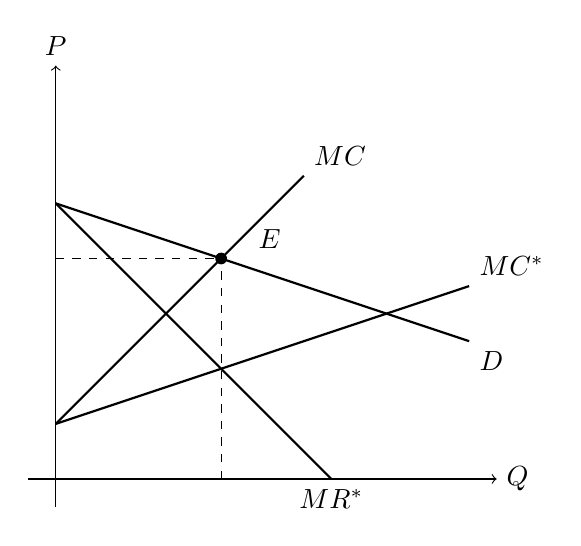
\begin{tikzpicture}[scale = 0.7]
                % Axes
                \draw[->] (-0.5,0) -- (8,0) node[right] {$Q$}; % Horizontal axis
                \draw[->] (0,-0.5) -- (0,7.5) node[above] {$P$}; % Vertical axis

                % Demand Curve (D_1) - passes through (0,5), (3,4), and (7.5,2.5)
                \draw[thick] (0,5) -- (7.5,2.5) node[below right] {$D$};
                % Marginal Revenue (MR_1) - passes through (0,5), (3,2), and (5,0)
                \draw[thick] (0,5) -- (5,0) node[below] {$MR^{*}$};

                % Supply Curve under competition (S^c) - passes through (0,1), (3,4), and (4.5,5.5)
                \draw[thick] (0,1) -- (4.5,5.5) node[above right] {$MC$};

                % Supply Curve under monopoly (S^m) - passes through (0,1), (3,2), and (7.5,3.5)
                \draw[thick] (0,1) -- (7.5,3.5) node[above right] {$MC^{*}$};

                % Equilibrium point (E_1) - intersection of D_1 and S^c at (3,4)
                \node[circle, fill, inner sep=1.5pt] (E1) at (3,4) {};
                \node[above right] at (E1) {$\quad E$};
                \draw[dashed] (3,0) -- (3,4);
                \draw[dashed] (0,4) -- (3,4);
            \end{tikzpicture}
            \caption{Step 1: Observable equivalence holds.}
            \label{fig:identification_example_step_1}
        \end{subfigure}
        \hfill
        \begin{subfigure}[b]{0.45\textwidth}
            \centering
            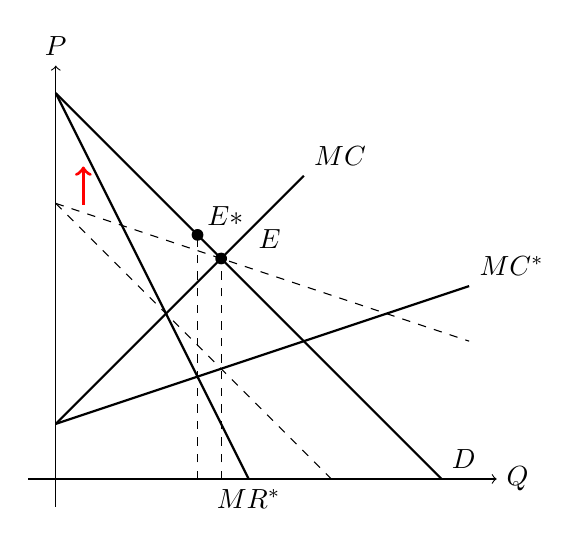
\begin{tikzpicture}[scale = 0.7]
                % Axes
                \draw[->] (-0.5,0) -- (8,0) node[right] {$Q$}; % Horizontal axis
                \draw[->] (0,-0.5) -- (0,7.5) node[above] {$P$}; % Vertical axis

                % Demand Curve (D_1) - passes through (0,5), (3,4), and (7.5,2.5)
                \draw[dashed] (0,5) -- (7.5,2.5) ;
                % Marginal Revenue (MR_1) - passes through (0,5), (3,2), and (5,0)
                \draw[dashed] (0,5) -- (5,0);


                % Shifted Demand Curve (D_1 shifted)
                \draw[thick] (0,7) -- (7,0) node[above right] {$D$};
                % Shifted MR (MR_1 shifted)
                \draw[thick] (0,7) -- (3.5,0) node[below] {$MR^{*}$};

                \draw[-<, very thick, red] (0.5,5) to[out=270,in=90] (0.5,5.5);


                % Supply Curve under competition (S^c) - passes through (0,1), (3,4), and (4.5,5.5)
                \draw[thick] (0,1) -- (4.5,5.5) node[above right] {$MC$};

                % Supply Curve under monopoly (S^m) - passes through (0,1), (3,2), and (7.5,3.5)
                \draw[thick] (0,1) -- (7.5,3.5) node[above right] {$MC^{*}$};

                % Equilibrium point (E_1) - intersection of D_1 and S^c at (3,4)
                \node[circle, fill, inner sep=1.5pt] (E1) at (3,4) {};
                \node[above right] at (E1) {$\quad E$};
                \draw[dashed] (3,0) -- (3,4);

                % Equilibrium point (E_2) - intersection of D_1 and S^c at (7/2,9/2)
                \node[circle, fill, inner sep=1.5pt] (E2) at (18/7,7 - 18/7) {};
                \node[above right] at (E2) {$E{*}$};
                \draw[dashed] (18/7,0) -- (18/7,7 - 18/7);
            \end{tikzpicture}
            \caption{Step 2: Demand rotation changes $D$ and $MR^{*}$, but $E$ remains the same.}
            \label{fig:identification_example_step_2}
        \end{subfigure}
        \begin{subfigure}[b]{0.5\textwidth}
            \centering
            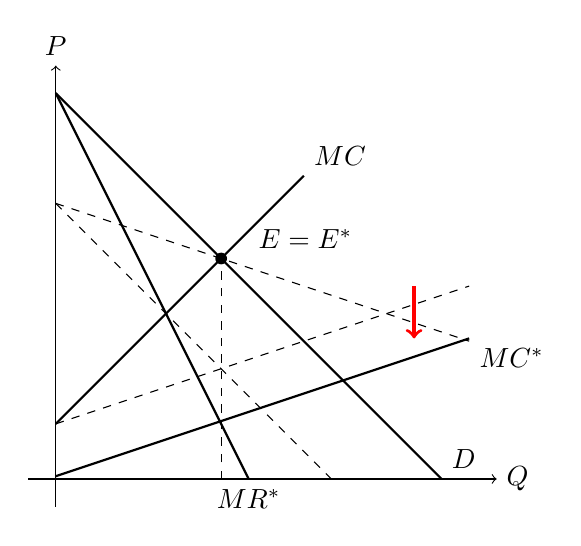
\begin{tikzpicture}[scale = 0.7]
                % Axes
                \draw[->] (-0.5,0) -- (8,0) node[right] {$Q$}; % Horizontal axis
                \draw[->] (0,-0.5) -- (0,7.5) node[above] {$P$}; % Vertical axis

                % Demand Curve (D_1) - passes through (0,5), (3,4), and (7.5,2.5)
                \draw[dashed] (0,5) -- (7.5,2.5) ;
                % Marginal Revenue (MR_1) - passes through (0,5), (3,2), and (5,0)
                \draw[dashed] (0,5) -- (5,0);

                % Shifted Demand Curve (D_1 shifted)
                \draw[thick] (0,7) -- (7,0) node[above right] {$D$};
                % Shifted MR (MR_1 shifted)
                \draw[thick] (0,7) -- (3.5,0) node[below] {$MR^{*}$};

                % Supply Curve under competition (S^c) - passes through (0,1), (3,4), and (4.5,5.5)
                \draw[thick] (0,1) -- (4.5,5.5) node[above right] {$MC$};

                % Supply Curve under monopoly (S^m) - passes through (0,1), (3,2), and (7.5,3.5)
                \draw[dashed] (0,1) -- (7.5,3.5);
                \draw[->, very thick, red] (6.5,3.5) -- (6.5,2.55);

                % Supply Curve under monopoly (S^m) - passes through (0,1), (3,2), and (7.5,3.5)
                \draw[thick] (0,0.05) -- (7.5,2.55) node[below right] {$MC^{*}$};

                % Equilibrium point (E_1) - intersection of D_1 and S^c at (3,4)
                \node[circle, fill, inner sep=1.5pt] (E1) at (3,4) {};
                \node[above right] at (E1) {$\quad E = E^{*}$};
                \draw[dashed] (3,0) -- (3,4);

            \end{tikzpicture}
            \caption{Step 3: $MC^{*}$ should change along with the demand rotation to keep $E = E^{*}$.}
            \label{fig:identification_example_step_3}
        \end{subfigure}
    \end{center}
    \caption{Intuition of the demand rotation instrument}
    \label{fig:identification_example}
    \vspace{2mm}
    \footnotesize
    Note: The figures illustrate the intuition of how the demand rotation instrument works to identify the conduct parameter.
    $MC$ is the true marginal cost function, and $MC^{*}$ is the marginal cost function that rationalizes the monopoly conduct.
    Step 1 illustrates the non-identification result.
    In step 2, the demand rotation changes the intercept and slope of the demand function without changing the equilibrium point under the true model, but changes the equilibrium point under the monopoly.
    Step 3 illustrates that to keep the equilibrium point under the monopoly, the marginal cost function should change along with the demand rotation, which is impossible because the marginal cost function is independent of the demand shifter.
\end{figure}





\section{Characterization of non-identification}\label{sec:non-identification_characterization}

In contrast, we can also define the identification of the conduct parameter and marginal cost function:
\begin{definition}\label{def:identification}
    Identification implies that for any two distinct pairs of conduct parameter and any marginal cost function, denoted as $(\theta, MC)$ and $(\theta^{*}, MC^{*})$, there exists a pair of demand shifter $X^{d}$ and $X^{s}$ where the equilibrium quantity $Q^e$ is different, that is, $h_q(X^{d}, X^{s}) \ne h_q^{*}(X^{d}, X^{s})$.
\end{definition}
The intuition is that identification means that given an economic condition, any different conduct parameters and marginal cost functions cannot lead to the same equilibrium quantity, that is, violates the observable equivalence of the equilibrium quantity.


Hereafter, we show that the identification result in \citet{lau1982identifying} is incorrect by providing a counterexample where a separable demand function induces identification.
Before proving the counterexample, we provide a lemma that characterizes the non-identification.

\begin{lemma}\label{lemma:non-identification_transformation}
    Non-identification implies that for any $Q^e$, $X^{d}$, and $X^{s}$,
    \begin{align}
        \frac{\partial MC^{*}}{\partial Q}(Q^e, X^{s}) = D_i(Q^e, X^{d}) + C_i(Q^e, X^{d})\frac{\partial MC}{\partial Q}(Q^e, X^{s}), \label{eq:mc_transformation}
    \end{align}
    where
    \begin{align}
        C_i(Q^e, X^{d}) \equiv \frac{\frac{\partial P}{\partial X^{d}_i}(Q^e, X^{d}) + \theta^{*} Q\frac{\partial^2 P}{\partial X^{d}_{i}\partial Q}(Q^e, X^{d}) }{\frac{\partial P}{\partial X^{d}_i}(Q^e, X^{d}) + \theta Q\frac{\partial^2 P}{\partial X^{d}_{i}\partial Q}(Q^e, X^{d}) },\label{eq:ratio_marginal_revenue}
    \end{align}
    and
    \begin{align}
        D_i(Q^e, X^{d}) \equiv\frac{(\theta^{*} - \theta)\frac{\partial }{\partial Q}\left[Q\frac{\partial P}{\partial Q}(Q^e, X^{d}) \frac{\partial P}{\partial X^{d}_i}(Q^e, X^{d})\right]}{\frac{\partial P}{\partial X^{d}_i}(Q^e, X^{d}) + \theta Q\frac{\partial^2 P}{\partial X^{d}_{i}\partial Q}(Q^e, X^{d})}.\label{eq:intercation_derivative_demand}
    \end{align}
\end{lemma}
See Appendix \ref{appendix:proof} for the proof.
This implies that given any conduct parameters $\theta$ and $\theta^{*}$ and a marginal cost function $MC$, marginal cost function $MC^{*}$ can be constructed based on \eqref{eq:mc_transformation}.
However, \eqref{eq:mc_transformation} does not necessary leads to a valid marginal cost function.
Note that $C_i(Q^e, X^{d})$ and $D_i(Q^e, X^{d})$ are functions of $Q^e$ and $X^{d}$, and hence by integrating \eqref{eq:mc_transformation} with respect to $Q$, $MC^{*}$ can be a function of $X^{d}$.
However, this violates the Assumption \ref{assumption:exclusive_shifters}.
Therefore, to have a valid marginal cost function $MC^{*}$, $C_i(Q^e, X^{d})$ and $D_i(Q^e, X^{d})$ should be independent of $X^{d}$.

To see how \eqref{eq:mc_transformation} relates to the identification, we consider the following examples.
Example \ref{example:bresnahan_1982} uses the inverse demand function in Section \ref{sec:identification_example} and shows that the conduct parameter is not identified because the $MC^{*}$ can be independent form the demand shifter $X^{d}$.
Example \ref{example:demand_counterexample} uses the inverse demand function in Section \ref{sec:identification_example} and shows for any marginal cost function $MC$, we cannot construct a $MC^{*}$ that is observationally equivalent to $MC$ and is independent form the demand shifter $X^{d}$.

\begin{example}\label{example:bresnahan_1982}
    Consider a linear demand such that
    \begin{align}
        P(Q^e, X^{d}) = \alpha_0 - \alpha_1Q + \alpha_2X^{d}.
    \end{align}
    Then, \eqref{eq:mc_transformation} is given as
    \begin{align}
        \frac{\partial MC^{*}}{\partial Q}(Q^e, X^{s}) = (\theta^{*} - \theta)\alpha_1 + \frac{\partial MC}{\partial Q}(Q^e, X^{s}).
    \end{align}
    This implies that $MC^{*}$ can be independent of $X^{d}$ and the following $MC^{*}$ leads to observationally equivalent to $MC$:
    \begin{align}
        MC^{*}(Q^e, X^{s}) = (\theta^{*} - \theta)\alpha_1Q + MC(Q^e, X^{s}).
    \end{align}
\end{example}

\begin{example}\label{example:demand_counterexample}
    Consider the linear demand given by \eqref{eq:demand_counterexample}.
    Then, \eqref{eq:mc_transformation} is given by
    \begin{align}
        \frac{\partial MC^{*}}{\partial Q}(Q^e, X^{s}) = (\theta^{*} - \theta)(-\alpha_1 + \alpha_3X^{d}) +  \frac{\alpha_2 + \theta\alpha_3Q^e}{\alpha_2 + \theta^{*}\alpha_3Q^e}\frac{\partial MC}{\partial Q}(Q^e, X^{s}).
    \end{align}
    This implies that any new marginal cost function $MC^{*}$ that is observationally equivalent to the given marginal cost function $MC$ should depend on the demand shifter, which is not allowed by the Assumption \ref{assumption:exclusive_shifters}.
    Section \ref{sec:identification_example} considers the case with linear marginal cost function, but this intuition holds for any marginal cost function $MC$.
\end{example}



\section{Characterization of identification}\label{sec:identification_characterization}


Because we are also interested in the identification of the conduct parameter, the violation of \eqref{eq:mc_transformation} implies that the identification.
We state the contraposition of Lemma \ref{lemma:non-identification_transformation}.
\begin{corollary}
    For any two distinct pairs of conduct parameter and marginal cost function, $(\theta, MC)$ and $(\theta^{*}, MC^{*})$, if there is a combination of $Q^e$, $X^{d}$, and $X^{s}$ such that \eqref{eq:lambda_foc_demand} does not hold, the conduct parameter and the marginal cost function are identified.
\end{corollary}



So far, we have not discussed the identification result in \citet{lau1982identifying}.
From \eqref{eq:ratio_marginal_revenue} and \eqref{eq:intercation_derivative_demand}, \eqref{eq:mc_transformation} cannot be well defined when 
\begin{align}
    \frac{\partial P}{\partial X^{d}_i}(Q^e, X^{d}) + \theta Q\frac{\partial^2 P}{\partial X^{d}_{i}\partial Q}(Q^e, X^{d}) = 0.
\end{align}








\begin{proposition}
    When the inverse demand function is given by \eqref{eq:demand_separable}, \eqref{eq:lambda_foc_demand} is violated, and hence the conduct parameter is identified.
\end{proposition}

\begin{proof}
    Suppose that $\theta = 0$.
    Then, $C(Q^e, X^{d}) = 0$ if $\frac{\partial P}{\partial X^{d}_{i}} =  0$.
    However, this violates Assumption \ref{assumption:exclusive_shifters}.
    Thus, when $\theta = 0$, $C(Q^e, X^{d}) = 0$ cannot happen.


    Suppose that $\theta \ne 0$.
    \begin{align}
        \frac{\partial P}{\partial X^{d}_i}(Q^e, X^{d}) + \theta\frac{\partial^2 P}{\partial Q\partial X^{d}_{i}}(Q^e, X^{d})Q = 0.
    \end{align}
    Here, we swap the order of differentiation by Assumption \ref{assumption:twice_differentiable}.
    Let $u_i(Q^e, X^{d}) \equiv \frac{\partial P}{\partial X^{d}_i}(Q^e, X^{d})$.
    Then, it becomes a ordinary differential equation for $u_i(Q^e, X^{d})$:
    \begin{align}
       u_i(Q^e, X^{d}) = -\theta Q\frac{\partial u_i}{\partial Q}(Q^e, X^{d}).
    \end{align}



\end{proof}

















\section{Checking sufficiency of separability}

Suppose that the inverse demand function is separable and given by \eqref{eq:demand_separable}.

For the sake of a contradiction, suppose that the conduct parameter is identified.
In this case, for any distinct pairs of the conduct parameter and the marginal cost, at least one equilibrium quantity $Q^e$ violates the condition \eqref{eq:lambda_foc_demand}.
Additionally, $Q^e$ should be realized as an equilibrium quantity for any pair of the conduct parameter and the marginal cost.
Nevertheless, the data does not have the quantity by which the researcher can see the violation of the observable equivalence.

In the following, we consider two cases where the observable equivalence is violated.
The first case is when one side is zero and the other is nonzero at the equilibrium quantity.
The second case is when both sides are nonzero at the equilibrium quantity.

\subsection{Case 1: one side is zero and the other is nonzero at the equilibrium quantity}
Given an inverse demand function, suppose that there is a pair of $\hat{Q}$, $\hat{X}^{d}$, and $\hat{X}^{s}$ such that 
\begin{align}
    \frac{\partial P}{\partial X^{d}_i}(\hat{Q}, r(\hat{X}^{d})) + \theta\frac{\partial^2 P}{\partial X^{d}_{i}\partial Q}(\hat{Q}, r(\hat{X}^{d}))\hat{Q}  \ne 0,\label{eq:case1_left}\\
    \frac{\partial P}{\partial X^{d}_i}(\hat{Q}, r(\hat{X}^{d})) + \theta^{*}\frac{\partial^2 P}{\partial X^{d}_{i}\partial Q}(\hat{Q}, r(\hat{X}^{d}))\hat{Q}  = 0.\label{eq:case1_right}
\end{align}
In this case, the observable equivalence is violated because the left-hand side is nonzero but the right-hand side is zero at the equilibrium quantity.


\begin{lemma}
    Given the inverse demand function, if \eqref{eq:case1_right} does not hold for any $Q$, $X^{d}$, there could be a marginal cost function under which $\hat{Q}$ does not arise as an equilibrium quantity.
\end{lemma}


\begin{proof}
    Note that the equation is equivalent to
    \begin{align}
        \frac{\partial}{\partial X^{d}_i}\left( P(\hat{Q}, r(X^{d})) + \theta\frac{\partial P}{\partial Q}(\hat{Q}, r(X^{d}))\hat{Q}\right) = 0.
    \end{align}
    The inside of the bracket is the marginal revenue function evaluated at the equilibrium quantity, and hence the equation implies that the marginal revenue does not depend on the demand shifter $X^{d}_i$.
    Thus, we can define the marginal revenue function $S(Q)$ depending only on quantity.
    As the inverse demand function is given, $S$ is also known.
    In this case, $\hat{Q}$ solves the first-order condition for the marginal cost function $MC(Q^e, X^{s})$.
    \begin{align}
        s(\hat{Q}) =  MC(\hat{Q}, X^{s}). \label{eq:case1_mc_foc}
    \end{align}
    Note that given $\hat{Q}$, the left-hand side is a constant and the right-hand side is a function of $X^{s}$.
    Because we assume that the marginal cost is twice continuously differentiable, the intermediate value theorem implies that given $\hat{Q}$, there exists a $\hat{X}^{s}$ that solve \eqref{eq:case1_mc_foc} when the range of the marginal cost includes $S(\hat{Q})$.    
    However, this does not hold for any marginal cost function.
    For example, when the inverse demand function is $P(Q^e, X^{d}) = Q^{-\frac{1}{\theta}}r(X^{d})$.
    Then, \eqref{eq:case1_mc_foc} becomes
    \begin{align}
        0 = MC(\hat{Q}, X^{s}).
    \end{align}
    When the range of the marginal cost function does not include zero, we cannot solve the equation for any $X^{s}$ given $\hat{Q}$.
\end{proof}



Now, consider the case where \eqref{eq:case1_right} holds for any $Q$, $X^{d}$.
In this case, the equation is regarded as a partial differential equation of $P(Q, r(X^{d}))$.
When the inverse demand function does not include any term relating to $X^{d}$, \eqref{eq:case1_right} is automatically satisfied for any $Q$, $X^{d}$.
However, in this case, \eqref{eq:case1_left} cannot be nonzero for any $Q$, $X^{d}$, which is a contradiction.
Thus, the inverse demand function should include a term relating to $X^{d}$.
Assume that the inverse demand function has a separable form such that $P(Q, r(X^{d})) = g(Q)r(X^{d}) + s(Q)$.

By substituting the separable function into the differential equation, we have 
\begin{align}
   0 & =  g(Q) r_i(X^{d}) + \theta g'(Q)r_i(X^{d}) Q\\
   & = r_i(X^{d})( g(Q) + \theta g'(Q)Q).
\end{align}
where $r_i(X^{d})$ is the derivative of $r(X^{d})$ with respect to $X^{d}_i$.
When $r_i(X^{d}) = 0$, $r(X^{d})$ should be a constant function, which implies that the inverse demand does not depend on the demand shifter $X^{d}$.
However, we already exclude this case, and hence we assume that $r_i(X^{d}) \ne 0$.
Therefore, we have 
\[g(Q) + \thetag'(Q)Q = 0.\]
This equation is an ordinary differential equation of $Q$ of $g(Q)$.
This can be written as
\begin{align}
    \frac{g'(Q)}{g(Q)} &= -\frac{1}{\theta} \frac{1}{Q}
\end{align}
Because the left-hand side is the derivative of $\log g(Q)$ and the right-hand side is also a derivative of $\log Q$, we have
\begin{align}
        \frac{d}{dQ} \log g(Q) &= -\frac{1}{\theta} \frac{d}{dQ} \log Q.
\end{align}
By integrating this over the domain of $Q$, we have
\begin{align}
    \int_{0}^\infty \frac{d}{dQ} \log g(Q) dQ &= -\frac{1}{\theta} \int_{0}^\infty  \frac{d}{dQ} \log Q dQ \\
    \log g(Q) &= -\frac{1}{\theta} \log Q + C\\
    g(Q) &= C Q^{-\frac{1}{\theta}},
\end{align}
where $C$ is the constant of integration.
Substituting this into $f$, we have 
\begin{align}
    P(Q^e, X^{d}) = C Q^{-\frac{1}{\theta}} h(X^{d}) + s(Q).
\end{align}
By redefining $r(X^{d}) = Cr(X^{d})$, we have
\begin{align}
    P(Q^e, X^{d}) &= Q^{-\frac{1}{\theta}} r(X^{d}) + s(Q),
\end{align}
which is the same with \eqref{eq:identification_separable}.

Additionally, we need to check that \eqref{eq:case1_left} is nonzero for any $Q$, $X^{d}$.
By substituting the above inverse demand function into the left-hand side of \eqref{eq:lambda_foc_demand}, we have
\begin{align}
    \frac{\partial P}{\partial X^{d}_{i}}(Q^e, X^{d}) + \theta\frac{\partial^2 P}{\partial X^{d}_{i}\partial Q}(Q^e, X^{d})Q  &= Q^{-1/\theta} r_i(X^d) - \frac{\theta}{\theta^{*}} Q^{-1/\theta-1} r_i(X^d) Q\\
    &= Q^{-1/\theta} r_i(X^d) \left(1 - \frac{\theta}{\theta^{*}} \right).
\end{align}
This becomes zero if and only if $\theta= \theta^{*}$.
Hence, under the inverse demand function, \eqref{eq:case1_left} and \eqref{eq:case1_right} hold simultaneously for any $Q$, $X^{d}$.

On the other hand, when we have
\begin{align}
    \frac{\partial P}{\partial X^{d}_i}(\hat{Q}, \hat{X}^{d}) + \theta^{*}\frac{\partial^2 P}{\partial X^{d}_{i}\partial Q}(\hat{Q}, \hat{X}^{d})\hat{Q}  \ne  0,\\
    \frac{\partial P}{\partial X^{d}_i}(\hat{Q}, \hat{X}^{d}) + \theta\frac{\partial^2 P}{\partial X^{d}_{i}\partial Q}(\hat{Q}, \hat{X}^{d})\hat{Q}  = 0,
\end{align}
because $\lambda(Q, X^{d}, X^{s}) \ne 0$ for any $Q$, $X^{d}$, and $X^{s}$, the right-hand side of \eqref{eq:lambda_foc_demand} is nonzero.
Therefore, when the true inverse demand function is
\begin{align}
    P(Q^e, X^{d}) = Q^{-\frac{1}{\theta^{*}}} r(X^{d}) + s(Q),
\end{align}
the observable equivalence is always violated.






\section{Necessity of Separability}

From Lemma \ref{lemma:non-identification_transformation}, we know that the non-identification implies the condition \eqref{eq:lambda_foc_demand} holds for all $Q^e$, $X^{d}$, and $X^{s}$.
When the demand shifter is a scalar, from the argument in the previous section, by putting $r(X^{d}) = X^{d}$, we can identify the conduct parameter and the marginal cost function only when the inverse demand function has the form of \eqref{eq:identification_separable}.

When the demand shifter is a vector, \eqref{eq:lambda_foc_demand} implies that
\begin{align}
    (1 - \lambda(Q^e, X^{d}, X^{s}))\frac{\partial P}{\partial X^{d}_i}(Q^e, X^{d}) = (\lambda(Q^e, X^{d}, X^{s})\theta -  \theta^{*})\frac{\partial^2 P}{\partial X^{d}_i\partial Q}(Q^e, X^{d})Q^e.
\end{align}
Pick up $i$ and $j$-th elements of the demand shifter and by taking the ratio the above equation, we have
\begin{align}
    \frac{\frac{\partial P}{\partial X^{d}_{i}}(Q^e, X^{d})}{\frac{\partial P}{\partial X^{d}_{j}}(Q^e, X^{d})} & = \frac{ \frac{\partial^2 P}{\partial X^{d}_{i} \partial Q}(Q^e, X^{d})}{\frac{\partial^2 P}{\partial X^{d}_{j} \partial Q}(Q^e, X^{d})},
\end{align}
which is equivalent to \footnote{See \ref{omitted_calculation} for the detailed calculation.}
\begin{align}
    0 & = \left. \left(\frac{\frac{\partial P}{\partial X^{d}_{i}}(Q^e, X^{d})}{\frac{\partial P}{\partial X^{d}_{j}}(Q^e, X^{d})}\right)^{-1} \frac{\partial}{\partial Q} \left(\frac{\frac{\partial P}{\partial X^{d}_{i}}(Q^e, X^{d})}{\frac{\partial P}{\partial X^{d}_{j}}(Q^e, X^{d})}\right) \right|_{Q = Q^e}.
    \label{eq:derivative_separable}
\end{align}

Because $X^{d}$ is a vector of demand shifters that affect the inverse demand function, it is natural to think that $\frac{\partial P}{\partial X^{d}_{i}}(Q^e, X^{d}) \ne 0$ for all $i$ and for any $Q$.
Therefore, we should have
\begin{align}
    \frac{\frac{\partial P}{\partial X^{d}_{i}}(Q^e, X^{d})}{\frac{\partial P}{\partial X^{d}_{j}}(Q^e, X^{d})} \ne 0 \quad \forall i, j, Q.
\end{align}
Therefore, the first term in \eqref{eq:derivative_separable} is nonzero, which implies that the derivative with respect to $Q$ at $Q^e$ is zero;
\begin{align}
    \left. \frac{\partial}{\partial Q} \left(\frac{\frac{\partial P}{\partial X^{d}_{i}}(Q^e, X^{d})}{\frac{\partial P}{\partial X^{d}_{j}}(Q^e, X^{d})}\right) \right|_{Q = Q^e} = 0.
\end{align}
This is equivalent to the weak separability in \citet{goldmanNote1964}, and hence we can apply Theorem 2 in \citet{goldmanNote1964} to conclude that when $X^{d}$ is a vector, non-identification implies that the inverse demand function is a separable function such that $P(Q, r(X^{d}))$.


\section{Conclusion and discussion}

We present a counterexample to \citet{lau1982identifying}'s identification result, separability does not imply non-identification.
Our finding is that even though non-identification implies the separability of the inverse demand function, the class of separable inverse demand functions that leads to non-identification is more restricted than the class considered in \citet{lau1982identifying}.

Based on the recent literature on distinguishing firm conduct, this result is not surprising.
For example, in the differentiated product environment, \citet{berry2014identification}  use a broader variation in markets to distinguish conduct beyond demand rotation.
In our counterexample, to violate observable equivalence, we need a variation in $X^{d}$ and $X^{s}$ that leads to a specific equilibrium quantity.
Of course, homogeneous product settings are more restricted than differentiated product settings, but it sounds too strong to claim that any separable demand function is a necessary and sufficient condition for non-identification of the conduct parameter.
Rather, even though the true inverse demand function is separable, the variation in markets may help to identify the conduct parameter.

In this note, we have not investigated the exact class of separable inverse demand functions that leads to non-identification of the conduct parameter.
However, in practice, this does not matter much because to estimate the conduct parameter, the researcher uses a parametric assumption on the inverse demand function and the marginal cost function (e.g., \citet{okazaki2022excess} and \citet{matsumura2024loglinear}).
Even though the researcher wants to non-parametrically estimate the marginal cost function, at least a non-separable demand function leads to the identification of the conduct parameter.

\paragraph{Acknowledgments}
We thank Jeremy Fox for his invaluable comments.
This work was supported by JST ERATO Grant Number JPMJER2301, Japan.  


\newpage
\bibliographystyle{aer}
\bibliography{conduct_parameter.bib}

\appendix

\section{Proofs}\label{appendix:proof}

\subsection{Proof of Lemma \ref{lemma:non-identification_transformation}}
Assume that given $X^{d}$ and $X^{s}$, we can solve the first-order condition for the equilibrium quantity $Q^e$.
Then, by Assumption \ref{assumption:unique_equilibrium}, we can apply the implicit function theorem, and for the reduced-form equation $Q^e = h_q(X^{d}, X^{s})$, the derivative of $h$ with respect to the demand shifters and the cost shifters are
\begin{align}
    Dh_q(X^{d}, X^{s}) = \begin{pmatrix}
        \dfrac{\partial h_q}{\partial X^{d}_{1}}(X^{d}, X^{s})\\
        \vdots \\
        \dfrac{\partial h_q}{\partial X^{d}_{K_d}}(X^{d}, X^{s})\\[1em]
        \dfrac{\partial h_q}{\partial X^{s}_{1}}(X^{d}, X^{s})\\
        \vdots \\
        \dfrac{\partial h_q}{\partial X^{s}_{K_s}}(X^{d}, X^{s})
    \end{pmatrix} = \begin{pmatrix}
        -\dfrac{\frac{\partial F}{\partial X^{d}_{1}}(h_q(X^{d}, X^{s}), X^{d}, X^{s})}{\frac{\partial F}{\partial Q}(h_q(X^{d}, X^{s}), X^{d}, X^{s})}\\
        \vdots \\
        -\dfrac{\frac{\partial F}{\partial X^{d}_{K_d}}(h_q(X^{d}, X^{s}), X^{d}, X^{s})}{\frac{\partial F}{\partial Q}(h_q(X^{d}, X^{s}), X^{d}, X^{s})}\\[1.5em]
        -\dfrac{\frac{\partial F}{\partial X^{s}_{1}}(h_q(X^{d}, X^{s}), X^{d}, X^{s})}{\frac{\partial F}{\partial Q}(h_q(X^{d}, X^{s}), X^{d}, X^{s})}\\
        \vdots \\        
        -\dfrac{\frac{\partial F}{\partial X^{s}}(h_q(X^{d}, X^{s}), X^{d}, X^{s})}{\frac{\partial F}{\partial Q}(h_q(X^{d}, X^{s}), X^{d}, X^{s})}
    \end{pmatrix}.\label{eq:foc_derivative_demand_supply}
\end{align}
The derivatives of $F$ for each variable are
\begin{align}
    \frac{\partial F}{\partial X^{d}_i}(Q^e, X^{d}, X^{s}; \theta, MC) & =  \frac{\partial P}{\partial X^{d}_{i}}(Q^e, X^{d}) + \theta\frac{\partial^2 P}{\partial X^{d}_{i}\partial Q}(Q^e, X^{d})Q^e, \quad i = 1, \ldots, K_d,\\
    \frac{\partial F}{\partial X^{s}_i}(Q^e, X^{d}, X^{s}; \theta, MC) & =  -\frac{\partial MC}{\partial X^{s}_{i}}(Q^e, X^{s}), \quad i = 1, \ldots, K_s, \\
    \frac{\partial F}{\partial Q}(Q^e, X^{d}, X^{s}; \theta, MC) & = (1+\theta)\frac{\partial P}{\partial Q}(Q^e, X^{d}) + \theta Q^e\frac{\partial^2 P}{\partial Q^2}(Q^e, X^{d}) - \frac{\partial MC}{\partial Q}(Q^e, X^{s}).
\end{align}
Thus, the derivative of $h$ with respect to $X^{d}_i$ and $X^{s}_i$ are given as for $i = 1, \ldots, K_d$ and $i = 1, \ldots, K_s$,
\begin{align}
    \frac{\partial h_q}{\partial X^{d}_{i}}(X^{d}, X^{s}) = -\frac{\frac{\partial P}{\partial X^{d}_{i}}(Q^e, X^{d}) + \theta Q^e \frac{\partial^2 P}{\partial X^{d}_{i}\partial Q}(Q^e, X^{d}) }{(1+\theta)\frac{\partial P}{\partial Q}(Q^e, X^{d}) + \theta  Q^e\frac{\partial^2 P}{\partial Q^2}(Q^e, X^{d}) - \frac{\partial MC}{\partial Q}(Q^e, X^{s})}, \label{eq:foc_derivative_demand}
\end{align}
and
\begin{align}
    \frac{\partial h_q}{\partial X^{s}_{i}}(X^{d}, X^{s}) & = \frac{\frac{\partial MC}{\partial X^{s}_{i}}(Q^e, X^{s})}{(1+\theta)\frac{\partial P}{\partial Q}(Q^e, X^{d}) + \theta  Q^e\frac{\partial^2 P}{\partial Q^2}(Q^e, X^{d}) - \frac{\partial MC}{\partial Q}(Q^e, X^{s})}. \label{eq:foc_derivative_supply}
\end{align}

% Use the definition of non-identification
Note that the same argument can be applied to the first-order condition \eqref{eq:foc_beta} of the alternative model.
Recall that the non-identification implies that $Q^e = h_q(X^{d}, X^{s}) = h_q^{*}(X^{d}, X^{s})$ for all $X^{d}$ and $X^{s}$, and hence we must have
\begin{align}
    Dh_q^{*}(X^{d}, X^{s}) = Dh_q(X^{d}, X^{s}) \quad \forall X^{d}, X^{s}. \label{eq:observale_equivalence_derivative}
\end{align}
From \eqref{eq:foc_derivative_demand_supply}, this implies that for all $Q^e$, $X^{d}$, and $X^{s}$,
\begin{align}
    \begin{pmatrix}
        \frac{\partial F}{\partial X^{d}_{1}}(Q^e, X^{d}, X^{s}; \theta^{*}, MC^{*})\\
        \vdots \\
        \frac{\partial F}{\partial X^{d}_{K_d}}(Q^e, X^{d}, X^{s}; \theta^{*}, MC^{*})\\
        \frac{\partial F}{\partial X^{s}_{1}}(Q^e, X^{d}, X^{s}; \theta^{*}, MC^{*})\\
        \vdots \\
        \frac{\partial F}{\partial X^{s}_{K_s}}(Q^e, X^{d}, X^{s}; \theta^{*}, MC^{*})
    \end{pmatrix}
    = \lambda(Q^e, X^{d}, X^{s})
    \begin{pmatrix}
        \frac{\partial F}{\partial X^{d}_{1}}(Q^e, X^{d}, X^{s}; \theta, MC)\\
        \vdots \\
        \frac{\partial F}{\partial X^{d}_{K_d}}(Q^e, X^{d}, X^{s}; \theta, MC)\\
        \frac{\partial F}{\partial X^{s}_{1}}(Q^e, X^{d}, X^{s}; \theta, MC)\\
        \vdots \\
        \frac{\partial F}{\partial X^{s}_{K_s}}(Q^e, X^{d}, X^{s}; \theta, MC)
    \end{pmatrix},\label{eq:foc_derivative_demand_supply_lambda}
\end{align}
where $\lambda(Q^e, X^{d}, X^{s})$ is defined as
\begin{align}
    \lambda(Q^e, X^{d}, X^{s}) \equiv \frac{(1+\theta^{*})\frac{\partial P}{\partial Q}(Q^e, X^{d}) + \theta^{*} Q^e\frac{\partial^2 P}{\partial Q^2}(Q^e, X^{d}) - \frac{\partial MC^{*}}{\partial Q}(Q^e, X^{s})}{(1+\theta)\frac{\partial P}{\partial Q}(Q^e, X^{d}) + \theta Q^e\frac{\partial^2 P}{\partial Q^2}(Q^e, X^{d}) - \frac{\partial MC}{\partial Q}(Q^e, X^{s})}. \label{eq:lambda_foc}
\end{align}
Assumption \ref{assumption:unique_equilibrium} guarantees that $\lambda(Q^e, X^{d}, X^{s})$ is nonzero and finite.
From the first $K_d$ rows in \eqref{eq:foc_derivative_demand_supply_lambda}, we have for $i = 1, \ldots, K_d$,
\begin{align}
    &\frac{\partial P}{\partial X^{d}_{i}}(Q^e, X^{d}) + \theta^{*} Q^e \frac{\partial^2 P}{\partial X^{d}_{i}\partial Q}(Q^e, X^{d})\\  
    &= \lambda(Q^e, X^{d}, X^{s})\left[ \frac{\partial P}{\partial X^{d}_{i}}(Q^e, X^{d}) + \theta Q^e \frac{\partial^2 P}{\partial X^{d}_{i}\partial Q}(Q^e, X^{d}) \right].
\end{align}
Therefore, by rearranging the terms, we have
\begin{align}
    &\frac{\frac{\partial P}{\partial X^{d}_i}(Q^e, X^{d}) + \theta^{*}\frac{\partial^2 P}{\partial X^{d}_{i}\partial Q}(Q^e, X^{d})Q^e }{\frac{\partial P}{\partial X^{d}_i}(Q^e, X^{d}) + \theta\frac{\partial^2 P}{\partial X^{d}_{i}\partial Q}(Q^e, X^{d})Q^e}\\
    &\quad = \frac{(1+\theta^{*})\frac{\partial P}{\partial Q}(Q^e, X^{d}) + \theta^{*} Q^e\frac{\partial^2 P}{\partial Q^2}(Q^e, X^{d}) - \frac{\partial MC^{*}}{\partial Q}(Q^e, X^{s})}{(1+\theta)\frac{\partial P}{\partial Q}(Q^e, X^{d}) + \theta Q^e\frac{\partial^2 P}{\partial Q^2}(Q^e, X^{d}) - \frac{\partial MC}{\partial Q}(Q^e, X^{s})}. \label{eq:lambda_foc_demand}
\end{align}


From \eqref{eq:lambda_foc_demand}, we have
\begin{align}
    &\frac{\partial MC^{*}}{\partial Q}(Q^e, X^{s}) - \frac{\frac{\partial P}{\partial X^{d}_i}(Q^e, X^{d}) + \theta^{*} Q\frac{\partial^2 P}{\partial X^{d}_{i}\partial Q}(Q^e, X^{d}) }{\frac{\partial P}{\partial X^{d}_i}(Q^e, X^{d}) + \theta Q\frac{\partial^2 P}{\partial X^{d}_{i}\partial Q}(Q^e, X^{d}) }\frac{\partial MC}{\partial Q}(Q^e, X^{s})\\
    & =  (1+ \theta^{*}) \frac{\partial P}{\partial Q}(Q^e, X^{d}) + \theta^{*} Q\frac{\partial^2 P}{\partial Q^2}(Q^e, X^{d})\\
    &\quad - \frac{\frac{\partial P}{\partial X^{d}_i}(Q^e, X^{d}) + \theta^{*} Q\frac{\partial^2 P}{\partial X^{d}_{i}\partial Q}(Q^e, X^{d}) }{\frac{\partial P}{\partial X^{d}_i}(Q^e, X^{d}) + \theta Q\frac{\partial^2 P}{\partial X^{d}_{i}\partial Q}(Q^e, X^{d}) }\left[(1+ \theta) \frac{\partial P}{\partial Q}(Q^e, X^{d}) + \theta Q\frac{\partial^2 P}{\partial Q^2}(Q^e, X^{d})\right].\label{eq:mc_transformation_1}
\end{align}
The right-hand side is written as
\begin{align}
    & (1+ \theta^{*})\frac{\partial P}{\partial Q} + \theta^{*} Q\frac{\partial^2 P}{\partial Q^2} - \frac{\frac{\partial P}{\partial X^{d}_i}(Q^e, X^{d}) + \theta^{*} Q\frac{\partial^2 P}{\partial X^{d}_{i}\partial Q}(Q^e, X^{d}) }{\frac{\partial P}{\partial X^{d}_i}(Q^e, X^{d}) + \theta Q\frac{\partial^2 P}{\partial X^{d}_{i}\partial Q}(Q^e, X^{d}) }\left[(1+ \theta) \frac{\partial P}{\partial Q} + \theta Q\frac{\partial^2 P}{\partial Q^2}\right]\\
    &= \frac{1}{\frac{\partial P}{\partial X^{d}_i} + \theta\frac{\partial^2 P}{\partial X^{d}_{i}\partial Q}Q}\left[\left((1 + \theta^{*}) \frac{\partial P}{\partial Q} + \theta^{*} Q\frac{\partial^2 P}{\partial  Q^2}Q\right)\left(\frac{\partial P}{\partial X^{d}_i} + \theta Q\frac{\partial^2 P}{\partial X^{d}_{i}\partial Q}\right)\right]\\
    &\quad - \frac{1}{\frac{\partial P}{\partial X^{d}_i} + \theta\frac{\partial^2 P}{\partial X^{d}_{i}\partial Q}Q}\left[\left( (1 + \theta) \frac{\partial P}{\partial Q} + \theta Q\frac{\partial^2 P}{\partial Q^2}Q\right)\left(\frac{\partial P}{\partial X^{d}_i} + \theta^{*} Q\frac{\partial^2 P}{\partial X^{d}_{i}\partial Q}\right)\right]\\
    & = \frac{\theta^{*} - \theta}{\frac{\partial P}{\partial X^{d}_i} + \theta Q\frac{\partial^2 P}{\partial X^{d}_{i}\partial Q}}\left[\frac{\partial P}{\partial Q} \frac{\partial P}{\partial X^{d}_i} + Q \frac{\partial P}{\partial Q} \frac{\partial^2 P}{\partial X^{d}_i\partial Q} + Q\frac{\partial^2 P}{\partial Q^2} \frac{\partial P}{\partial X^{d}_i} \right]\\
    & = \frac{\theta^{*} - \theta}{\frac{\partial P}{\partial X^{d}_i} + \theta Q\frac{\partial^2 P}{\partial X^{d}_{i}\partial Q}}\frac{\partial}{\partial Q}\left[ Q \frac{\partial P}{\partial Q} \frac{\partial P}{\partial X^{d}_i} \right].
\end{align}
The last term is the derivative of $ \frac{\partial P}{\partial Q} \frac{\partial P}{\partial X^{d}_i}$ with respect to $Q$.
By using the definition of $C_i$ and $D_i$,  we have \eqref{eq:mc_transformation} from \eqref{eq:mc_transformation_1}.


\section{Omitted Calculations}\label{omitted_calculation}


\begin{align}
    \frac{\frac{\partial^2 P}{\partial X^{d}_{i} \partial Q}(Q^e, X^{d})}{\frac{\partial P}{\partial X^{d}_{i}}(Q^e, X^{d})}  & = \frac{\frac{\partial^2 P}{\partial X^{d}_{j} \partial Q}(Q^e, X^{d})}{\frac{\partial P}{\partial X^{d}_{j}}(Q^e, X^{d})}\\ 
    \frac{\partial }{\partial Q} \log\left( \frac{\partial P}{\partial X^{d}_{i}}(Q^e, X^{d})\right) &= \frac{\partial }{\partial Q} \log\left( \frac{\partial P}{\partial X^{d}_{j}}(Q^e, X^{d})\right)\\
    0& = \frac{\partial}{\partial Q}\log\left(\frac{\frac{\partial P}{\partial X^{d}_{i}}(Q^e, X^{d})}{\frac{\partial P}{\partial X^{d}_{j}}(Q^e, X^{d})}\right)
\end{align}
Note that we can exchange the order of partial derivative due to Young's theorem as $P$ is twice continuously differentiable.
Then, by the chain rule, we have
\begin{align}
    0 & = \left(\frac{\frac{\partial P}{\partial X^{d}_{i}}(Q^e, X^{d})}{\frac{\partial P}{\partial X^{d}_{j}}(Q^e, X^{d})}\right)^{-1} \frac{\partial}{\partial Q} \left(\frac{\frac{\partial P}{\partial X^{d}_{i}}(Q^e, X^{d})}{\frac{\partial P}{\partial X^{d}_{j}}(Q^e, X^{d})}\right).
\end{align}




Theorem \ref{theorem_lau} shows that when the inverse demand function takes the special form \eqref{eq:demand_separable}, the conduct parameter and the marginal cost function are identified.
However, the problem is that while we can identify the reduced-form function of the equilibrium quantity and the equilibrium price, when the true inverse demand satisfies \eqref{eq:demand_separable}, the inverse demand function cannot be identified.

Under the inverse demand function, the first-order condition is written as
\begin{align}
    \theta s'(Q)Q = MC(Q^e, X^{s}).
\end{align}
This implies that the equilibrium quantity does not depend on the demand shifter.
Therefore, the equilibrium price also does not depend on the demand shifter.
Therefore, their reduced forms also independent fo the demand shifter.
More formally, Lau's proof shows that when the inverse demand function takes the form, $\frac{\partial h}{\partial X_i^{d}}(Q^e, X^{d}) = 0$ under the true conduct parameter. 





In this case, while the inverse demand function depends on the demand shifter through $r$, the observed data does not provide any information about $r$ term.
Especially, any $r$ can rationalize the data, which prevent the researcher from identifying the inverse demand function.

Without identifying the inverse demand function, when the researcher pick arbitrary functions of 





\end{document}